% BEVFusion (nuScenes detection, ConvFuser) architecture and deployment partition.
% Compile: pdflatex bevfusion_architecture.tex  (or: tectonic bevfusion_architecture.tex)
\documentclass[tikz,border=8pt]{standalone}

\usepackage[T1]{fontenc}
\usetikzlibrary{arrows.meta, backgrounds, calc, fit, positioning, shapes.geometric}

\definecolor{camA}{HTML}{2A78D6}
\definecolor{lidA}{HTML}{1BAF7A}
\definecolor{fusA}{HTML}{EB6834}
\definecolor{heaA}{HTML}{6250D6}
\definecolor{inkA}{HTML}{262626}
\definecolor{mutA}{HTML}{6B6B6B}

\tikzset{
  base/.style={
    draw=inkA!70, line width=0.45pt, rounded corners=2.5pt,
    align=center, font=\small, inner sep=3pt,
    minimum height=1.05cm, text=inkA,
  },
  cam/.style={base, fill=camA!10, draw=camA!70},
  lid/.style={base, fill=lidA!10, draw=lidA!70},
  fus/.style={base, fill=fusA!12, draw=fusA!75},
  hea/.style={base, fill=heaA!10, draw=heaA!70},
  io/.style={base, fill=black!4, draw=inkA!55},
  arr/.style={-{Stealth[length=2.1mm,width=1.5mm]}, line width=0.6pt, draw=inkA!70},
  tag/.style={font=\scriptsize, text=mutA},
  unit/.style={draw=mutA!80, dashed, line width=0.5pt, rounded corners=5pt, inner sep=5pt},
}

\begin{document}
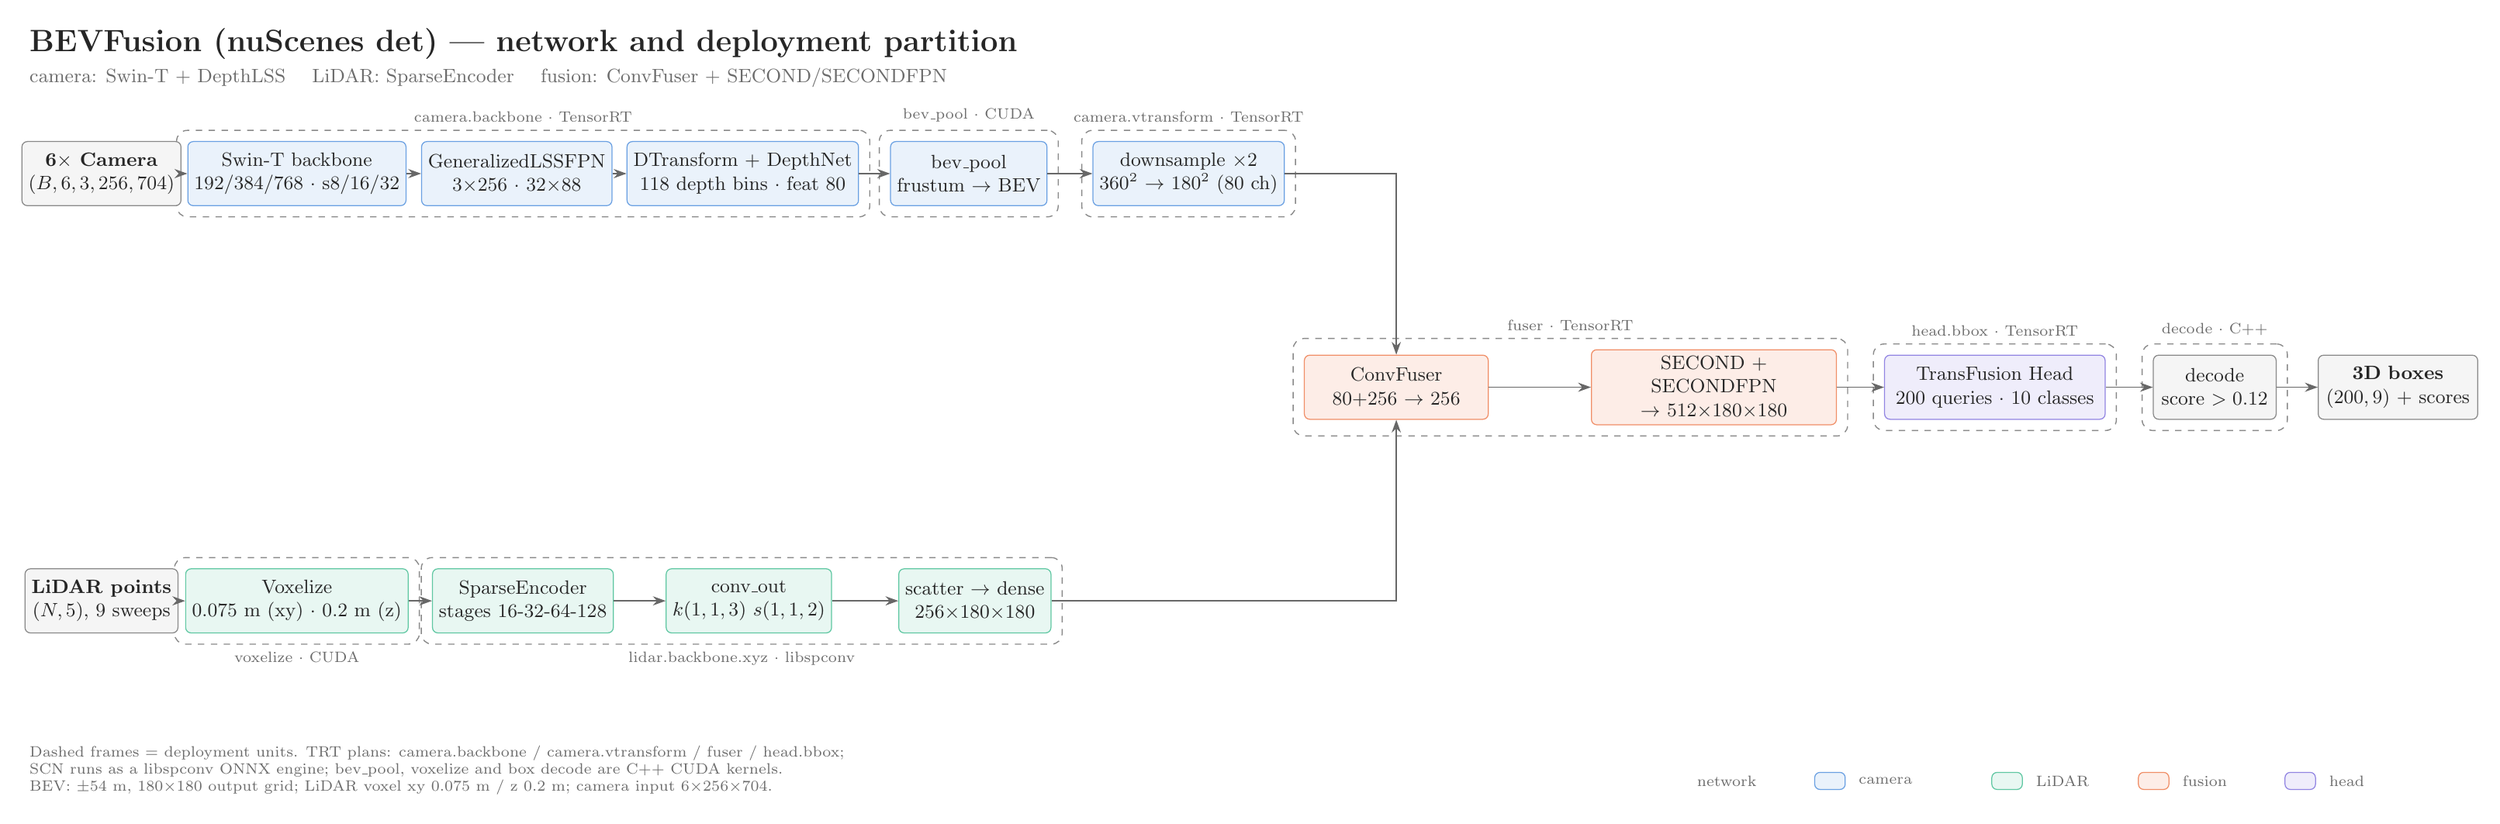
\begin{tikzpicture}

% ------------------------------------------------------------------ inputs
\node[io] (cin)  at (0,9.6)  {\textbf{6$\times$ Camera}\\$(B,6,3,256,704)$};
\node[io] (lin)  at (0,2.6)  {\textbf{LiDAR points}\\$(N,5)$, 9 sweeps};

% ------------------------------------------------------------------ camera
\node[cam] (swin)  at (3.2,9.6)  {Swin-T backbone\\192/384/768 $\cdot$ s8/16/32};
\node[cam] (fpn)   at (6.8,9.6)  {GeneralizedLSSFPN\\3$\times$256 $\cdot$ 32$\times$88};
\node[cam] (dtr)   at (10.5,9.6) {DTransform + DepthNet\\118 depth bins $\cdot$ feat 80};
\node[cam] (pool)  at (14.2,9.6) {bev\_pool\\frustum $\to$ BEV};
\node[cam] (down)  at (17.8,9.6) {downsample $\times$2\\360$^2$ $\to$ 180$^2$ (80 ch)};

\draw[arr] (cin)  -- (swin);
\draw[arr] (swin) -- (fpn);
\draw[arr] (fpn)  -- (dtr);
\draw[arr] (dtr)  -- (pool);
\draw[arr] (pool) -- (down);

% ------------------------------------------------------------------ lidar
\node[lid] (vox)   at (3.2,2.6)  {Voxelize\\0.075 m (xy) $\cdot$ 0.2 m (z)};
\node[lid] (scn)   at (6.9,2.6)  {SparseEncoder\\stages 16-32-64-128};
\node[lid] (cout)  at (10.6,2.6) {conv\_out\\$k(1,1,3)$ $s(1,1,2)$};
\node[lid] (dense) at (14.3,2.6) {scatter $\to$ dense\\256$\times$180$\times$180};

\draw[arr] (lin)   -- (vox);
\draw[arr] (vox)   -- (scn);
\draw[arr] (scn)   -- (cout);
\draw[arr] (cout)  -- (dense);

% ------------------------------------------------------------------ fusion / head
\node[fus, text width=2.8cm] (fuser)  at (21.2,6.1) {ConvFuser\\80+256 $\to$ 256};
\node[fus, text width=3.8cm] (dec)    at (26.4,6.1) {SECOND + SECONDFPN\\$\to$ 512$\times$180$\times$180};
\node[hea, text width=3.4cm] (head)   at (31.0,6.1) {TransFusion Head\\200 queries $\cdot$ 10 classes};
\node[io,  text width=1.8cm] (decode) at (34.6,6.1) {decode\\score $>0.12$};
\node[io,  text width=2.4cm] (out)    at (37.6,6.1) {\textbf{3D boxes}\\$(200,9)$ + scores};

\draw[arr] (down.east)  -| (fuser.north);
\draw[arr] (dense.east) -| (fuser.south);
\draw[arr] (fuser) -- (dec);
\draw[arr] (dec)   -- (head);
\draw[arr] (head)  -- (decode);
\draw[arr] (decode) -- (out);

% ------------------------------------------------------------------ deployment units
\begin{scope}[on background layer]
  \node[unit, fit=(swin)(fpn)(dtr), label={[tag]above:camera.backbone $\cdot$ TensorRT}] {};
  \node[unit, fit=(pool),          label={[tag]above:bev\_pool $\cdot$ CUDA}] {};
  \node[unit, fit=(down),          label={[tag]above:camera.vtransform $\cdot$ TensorRT}] {};
  \node[unit, fit=(vox),           label={[tag]below:voxelize $\cdot$ CUDA}] {};
  \node[unit, fit=(scn)(cout)(dense), label={[tag]below:lidar.backbone.xyz $\cdot$ libspconv}] {};
  \node[unit, fit=(fuser)(dec),    label={[tag]above:fuser $\cdot$ TensorRT}] {};
  \node[unit, fit=(head),          label={[tag]above:head.bbox $\cdot$ TensorRT}] {};
  \node[unit, fit=(decode),        label={[tag]above:decode $\cdot$ C++}] {};
\end{scope}

% ------------------------------------------------------------------ titles / notes
\node[anchor=north west, font=\Large\bfseries, text=inkA] at (-1.3,12.1)
  {BEVFusion (nuScenes det) --- network and deployment partition};
\node[anchor=north west, font=\small, text=mutA] at (-1.3,11.45)
  {camera: Swin-T + DepthLSS \quad LiDAR: SparseEncoder \quad fusion: ConvFuser + SECOND/SECONDFPN};

\node[anchor=north west, font=\scriptsize, text=mutA, align=left] at (-1.3,0.35)
  {Dashed frames = deployment units.  TRT plans: camera.backbone / camera.vtransform / fuser / head.bbox;\\
   SCN runs as a libspconv ONNX engine; bev\_pool, voxelize and box decode are C++ CUDA kernels.\\
   BEV: $\pm$54 m, 180$\times$180 output grid; LiDAR voxel xy 0.075 m / z 0.2 m; camera input 6$\times$256$\times$704.};

% ------------------------------------------------------------------ legend
\begin{scope}[shift={(26.0,-0.35)}]
  \node[tag, anchor=west] at (0,0) {network};
  \node[cam, minimum width=0.5cm, minimum height=0.28cm, inner sep=0pt] at (2.3,0) {};
  \node[tag, anchor=west] at (2.65,0) {camera};
  \node[lid, minimum width=0.5cm, minimum height=0.28cm, inner sep=0pt] at (5.2,0) {};
  \node[tag, anchor=west] at (5.55,0) {LiDAR};
  \node[fus, minimum width=0.5cm, minimum height=0.28cm, inner sep=0pt] at (7.6,0) {};
  \node[tag, anchor=west] at (7.95,0) {fusion};
  \node[hea, minimum width=0.5cm, minimum height=0.28cm, inner sep=0pt] at (10.0,0) {};
  \node[tag, anchor=west] at (10.35,0) {head};
\end{scope}

\end{tikzpicture}
\end{document}
